\documentclass[letterpaper,12pt]{article}
\date{\today}
\title{Tetris part 2}
\usepackage{geometry}
\usepackage{graphicx}
\usepackage[tikz]{bclogo}

\usepackage{../slides}
\geometry{left=2cm,right=2cm,top=1.5cm,bottom=1.5cm}
\usepackage[pdfusetitle]{hyperref}

\begin{document}
\begin{center}
    \Large{Tetric Part 2}
\end{center}
Last time we created a Piece class which could rotate. This time we want to implement 3 new methods for the Piece class for future use.

\begin{enumerate}
    \item \verb|getWidth()|.\\ This is simple. It should return the width of piece.
    \item \verb|getHeight()|.\\ Similarly, this method returns the height of the piece.
    \item \verb|getSkirt()|.\\This method returns an array which indicate the "bottom shape" of the piece. As long as the piece is wide, the skirt stores the lowest
    y value for each x value in the piece coordinate system. For example, the skirt of this piece below is \verb|[1,0,1]|.
    \\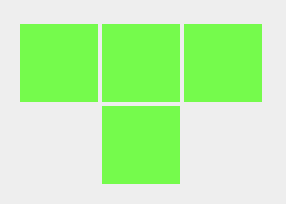
\includegraphics[scale=0.5]{skrt.png}
\end{enumerate}
 To complete this work, please download the reference implementation of
 \verb|Piece.java| and \verb|PieceTester.java| from
 \href{https://github.com/shawnma/geometry/tree/main/apcsa/tetris/piece}{https://github.com/shawnma/geometry/tree/main/apcsa/tetris/piece}, and implement the methods in \verb|Piece.java| with \verb|TODO|.
 \\ Note I made \verb|rotate()| private and created a new \verb|next()| method to get a rotated piece.
 \begin{lstlisting}[language=java]
 
    public int getWidth() {
        // TODO
        return 0;
    }

    public int getHeight() {
        // TODO
        return 0;
    }

    public int[] getSkirt() {
        // TODO
        return new int[3];
    }
 \end{lstlisting}
 Note, if you run the \verb|PieceTest.java|, the UI will show the width, height and skirt returned by code. please verify it shows the correct
 value for each possible pieces and submit the code.
 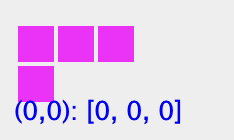
\includegraphics{size.png}

 \begin{bclogo}[logo=\bcattention, noborder=true]{Bonus}
Implement the methods in an optimized way by storing \verb|width|, \verb|height| and \verb|[]skirt| as member of the class so we don't
    need to compute them every time we call the getXXX method.
    
 \end{bclogo}
 
\end{document}
